\chapter[Contexte en biologie structurale]{Contexte, usages et enjeux en biologie structurale}
\minitoc
\cleardoublepage


\section{Liste des figures}

\begin{itemize}
	\item Transcription/traduction schématisées
	\item Tableau correspondance triplet ARN -> AA
	\item Illustrations des niveaux de structure
	\item Liaison peptidique avec angles dièdres et diagramme Ramachandran
	\item Cristallographie à différentes résolutions
	\item Champs de force et différence de précision
	\item Stéréoscopie / HMD / CAVE / ...
	\item Potentiels harmonique vs Morse
\end{itemize}

\section{Comprendre la cellule à l'échelle moléculaire}

L'étude des différents métabolismes régulant la vie des cellules, unité de base constituant l'ensemble des organismes vivants, peut être divisée en plusieurs sous-domaines caractérisés: par l'échelle à laquelle les phénomènes sont observés, par la nature des organismes étudiés et par les méthodes utilisés pour les étudier. Parmi ces sous-domaines, la biologie moléculaire s'intéresse à l'étude de la structure et des interactions entre biomolécules (ADN, ARN et protéines) et leur synthèse au sein de la cellule. Elle a pour but d'expliquer des phénomènes biologiques de grandes échelles d'un point de vue moléculaire. La biologie moléculaire se rapproche beaucoup de la biochimie à qui elle emprunte plusieurs techniques et idées. La biochimie s'intéresse plus spécifiquement à l'étude des phénomènes chimiques régissant les interactions entre les biomolécules. Autre discipline gravitant autour de l'étude des interactions, fonctions et structures des molécules, la biophysique possède une approche plus quantitative de la question et cherche à expliquer les phénomènes moléculaires grâce aux lois physiques régissant le reste du monde. A l'intersection de ces trois domaines d'études se trouve la biologie structurale, domaine spécifiquement intéressé aux structures mêmes des biomolécules, aux étapes permettant à une biomolécule d'acquérir une structure fonctionnelle et aux effets de la structure sur la fonction des biomolécules. C'est un domaine d'étude utilisant plusieurs techniques expérimentales et computationnelles, principalement basées sur des lois physiques, afin d'obtenir une description de précision atomique de la structure des molécules étudiées et de leur dynamique structurelle dans leur environnement cellulaire, impliquant donc les interactions qu'elles peuvent avoir avec d'autres biomolécules et la conséquence sur leur structure. La structure des biomolécules est au coeur de nombreuses recherches scientifiques car elle est directement liée à leur fonction \cite{lodish2000molecular}.
Il est possible de distinguer plusieurs familles de biomolécules: Les protéines, les acides nucléiques, les lipides, l'eau, etc. Elles ont en commun leur participation aux processus métaboliques de la cellule, indépendamment ou par des interactions plus ou moins complexes entre-elles. Notre étude porte majoritairement sur les biomolécules naturelles de grandes tailles, appelées également macromolécules, regroupant exclusivement les acides nucléiques et les protéines. Nous aurons une attention particulière sur les complexes protéiques même si la portée de nos recherches peut majoritairement s'étendre aux acides nucléiques.

\subsection{Les biomolécules, unités du vivant}

L'intégralité des informations ayant permis à un être vivant de posséder son apparence et son fonctionnement se retrouvent constitue l'information génétique. Le support de cette information génétique est portée par un type de biomolécules, l'\textbf{ADN}, permettant de stocker cette information et de la rendre accessible, sous certaines conditions et via certains processus complexes, dont l'interprétation se fera tout d'abord à l'échelle moléculaire, puis cellulaire, ensuite organique et finalement organismique.

Les processus impliqués dans la transformation de l'information génétique en composants fonctionnels dont les actions peuvent être quantifiables sont nombreux et complexes mais indispensables à la compréhension des mécanismes de la vie chez les êtres vivants. Dans cette première partie de chapitre, nous resterons à l'échelle moléculaire et nous essayerons de décrire brièvement le processus métabolique permettant de passer de l'information génétique porté par l'ADN à l'unité biologique fonctionnel que constituent l'ensemble des \textbf{protéines}.
Ce processus se caractérise par deux étapes principales, la transcription et la traduction. La transcription permet de transférer les informations contenues dans le noyau et portées par l'ADN vers le lieu de la traduction, à l'extérieur du noyau cellulaire, dans la zone appelée cytosplasme et constituant l'ensemble d'une cellule eucaryote en dehors du noyau. Ce transfert se fait grâce à l'ARN, un acide nucléique simple brin, qui est capable de traverser la paroi cellulaire au contraire de l'ADN, double brin sous forme d'hélice et donc structurellement trop gros pour traverser cette paroi. Lorsque les ARN parviennent aux organites cellulaires responsables de la traduction, les ribosomes, elles s'y lient et l'étape de traduction peut commencer. La traduction consiste à transformer l'information génétique de l'ADN, copiée par les ARN, pour former les protéines. Ces deux étapes indispensables à la formation des protéines sont résumées et illustrées dans la figure X.

\subsubsection{ADN}

L'Acide DésoxyriboNucléique (ADN) est une molécule biologique retrouvée dans toutes les cellules. C'est une suite précise de nucléotides, présents sous quatre formes distinctes et qui constituent la structure de l'ADN. Ils sont constitués d'une structure moléculaire commune constituée d'un sucre, le désoxyribose, et d'un groupe phosphate. A cette partie commune se lie une base azotée spécifique pouvant adopter 4 formes ((Adénine, Thymine, Guanine et Cytosine). Les nucléotides sont organisés le long de deux brins liés l'un à l'autre grâce à la complémentarité des nucléotides deux à deux. L'Adénine se liant à la Thymine et la Guanine pouvant se lier à la Cytosine. Ces deux brins prennent une structure hélicoïdale précise dans le noyau. Cette complémentarité des brins permet tout d'abord d'assurer une certaine résistance de la structure à la dégradation et, en cas d'endommagement d'un des deux brins, elle permet la réparation du brin intact. L'ADN est elle-même organisée en superstructures appelées chromosomes. Ces chromosomes permettent à l'ADN d'être plus compacte et régulent également leur transcription en ARN.
L'ADN est découpé en séquences codantes et non codantes, les séquences codantes seront directement impliqués dans la formation de protéines alors que les séquences non codantes ont un rôle de régulation ou de stabilité mais ne mènent de façon directe à aucune structure moléculaire.
Chez les eucaryotes (organismes pluricellulaires possédant un noyau dans la cellule), l'ADN est stockée dans le noyau et ne peut en sortir à cause de sa taille trop importante qui l'empêche de traverser la membrane nucléique. Le passage de l'information génétique du noyau vers le cytosplasme des cellules eucaryotes se fait donc grâce aux ARN.

\subsubsection{ARN}

L'Acide Ribonucléique (ARN) est une biomolécule structurellement proche de l'ADN comportant néanmoins quelques différences notables. La première se retrouve au niveau du sucre constituant chacun des nucléotides puisque le désoxyribose de l'ADN est remplacé par un ribose pour l'ARN. De plus, la Thymine présente dans l'ADN n'existe pas chez l'ARN et est remplacée par l'Uracile mais reste toujours complémentaire à l'Adénine. La seconde différence concerne la structuration des brins puisqu'on ne retrouve pas de structure en double brin chez l'ARN qui existe exclusivement sous forme de simple brin. Cette structure lui permet, sous certaines conditions, de traverser la membrane nucléique des noyaux des cellules eucaryotes.
En plus de ces différences structurelles L'ARN existe sous plusieurs formes, chacune avec un rôle bien précis. Ces différents ARNs sont présentés succinctement ci-dessous, le rôle des plus importants sera explicité dans la description des étapes de transcription et de traduction dans la section \ref{trans_trad}.
L'\textbf{ARNm}, ou ARN messager, est l'ARN responsable de la transmission de l'information génétique porté de l'ADN depuis le noyau jusqu'au cytoplasme. Il est créé pendant l’étape de transcription.
L'\textbf{ARNt}, ou ARN de transfert, sont des ARN de taille limitée (entre 70 et 100 nt) qui permettent le transport des acides aminés vers le ribosome lors de la traduction.
Les \textbf{ARN catalytiques} regroupent les ARN possédant un rôle catalytique dans la cellule. Ils interviennent par exemple pour des étapes d'épissage de l'ARNm pendant son étape de maturation, certains ARN de virus peuvent se cliver eux-mêmes et sont donc potentiellement indépendants alors que d'autres peuvent catalyser certaines réactions chimiques et de fixer certaines molécules.
Les \textbf{ARN guides} sont des ARN s'associant à des enzymes protéiques afin de diriger leurs actions vers des ARN ou des ADN de séquences complémentaires.
Les \textbf{ARN régulateurs} ont pour cible les ARNm sur lesquels ils se lient par complémentarité. Cette liaison peut empêcher la traduction de l'ARNm cible par les ribosomes ou bien agir sur la stabilité de l'ARNm régulant ainsi son expression (positivement ou négativement).

\subsubsection{Protéines}

Les protéines sont les biomolécules considérées comme les plus fonctionnelles puisque leurs rôles sont multiples au sein de la cellule mais également en dehors. Elles sont notamment impliquées dans: rôle \textit{structurel}, l'actine et le collagène assurent par exemple le maintien physique et structurel de la cellule ainsi que la résistance de la matrice extracellulaire, dans la \textit{mobilité}, les myosines permettent par exemple la contraction musculaire en se liant aux actines, dans le \textit{conditionnement de l'ADN}, l'ADN est enroulé autour de protéines appelées les histones, dans la régulation de l'expression génétique, les facteurs de transcription accompagnant l'ARN polymérase lors de la transcription sont des protéines, etc.

Une protéine est constituée d'une succession d'acides aminés. Au sein des protéines présents chez les êtres vivants, 22 acides aminés différents ont été identifiés. Parmi ces 22 acides aminés, 19 d'entre-eux ne sont constitués que de quatre atomes distincts: le carbone, l'hydrogène, l'oxygène et l'azote. Deux autres possèdent également un atome de soufre et enfin le dernier, plus rare, possède un atome de sélénium. Ces acides aminés possèdent une partie commune qui constitue, lorsqu'ils sont liés, la \textit{chaîne principale} ou squelette de la protéine. C'est au niveau de la chaîne latérale que les acides aminés sont liés entre-eux en formant une \textit{liaison peptidique}. Les différents acides aminés se différencient par une partie variante possédant 22 combinaisons et appelée la \textit{chaîne latérale}. La chaîne latérale des acides aminés donne lieu a des propriétés physico-chimiques différentes. Chaque acide aminé peut donc être représenté par la structure générique H$_{2}$N-HC\textit{R}-COOH, dans laquelle \textit{R} désigne la chaîne latérale. 
Il est possible de classer les acides aminés selon plusieurs critères, depuis leur taille jusque leur propriété hydrophobique (affinité avec l'eau) ou leur polarité. Il existe cependant un classement commun qui les regroupe en six groupes fonctionnels: Les acides aminés \textit{aliphatiques} (Glycine, Alanine, Valine, Leucine et Isoleucine), les acides aminés avec groupement \textit{hydroxyle, sulfurique ou sélénique} (Sérine, Thréonine, Méthionine, Cystéine et Sélénocystéine), les acides aminés \textit{cycliques} (Proline), les acides aminés \textit{aromatiques} (Phénylalanine, Tyrosine et Tryptophane), les acides aminés \textit{basiques} (Histidine, Lysine et Arginine) et enfin les acides aminés \textit{acides} et leurs \textit{amides} (Aspartate, Glutamate, Asparagine et Glutamine).

La séquence des acides aminés est appelée la \textbf{structure primaire} d'une protéine. Les séquences en acides aminés des protéines sont énoncés de façon à commencer de la partie Nter de la protéine, le premier acide aminé ne possédant donc qu'une liaison peptidique du côté de son groupement carbonyle alors que le dernier acide aminé n'est lui lié que du côté du groupement amide.
Les groupements amide (-NH) et carbonyle (-CO) du squelette peptidique, retrouvés au niveau de la chaîne principale des acides aminés, forment des liaisons hydrogènes qui vont entraîner la création de certains motifs structurant la protéines. Les motifs structuraux formés sont au nombre de 3: \textit{Hélices}, \textit{feuillets} et \textit{coudes} même si chaque motif possède cependant quelques variations structurales légères. L’enchaînement de ces motifs d'acides aminés est appelée la \textbf{structure secondaire} de la protéine. Bien que la structure secondaire soit stabilisée par des liaisons hydrogènes formée au niveau de la chaîne principale des acides aminés, cette structuration dépend également d'autres propriétés structurales dépendantes des contraintes énergétiques de la structure. Ces contraintes vont modifier les liaisons peptidiques au niveau de leurs angles dièdres $\phi$ et $\psi$ (angles composés par 2 plans définis par 4 atomes comme illustré dans la figure X). Il est possible d'extraire des valeurs d'angles dièdres propres à chaque structuration et on retrouve ces gammes de valeurs dans le diagramme de Ramachandran \cite{ramachandran1968conformation}.
Enfin, les protéines possèdent également des motifs plus importants, souvent le résultat de l'agencement dans l'espace des motifs de structures secondaires cités précédemment. C'est la \textbf{structure tertiaire} ou structure tridimensionnelle de la protéine. Cette structure est maintenue par différents types d'interactions. Les interactions \textit{covalentes} sont essentiellement le fait de ponts disulfures pouvant exister entre deux cystéines. Les interactions \textit{électrostatiques} regroupent les liaisons ioniques (entre cations et anions des chaînes latérales) et hydrogènes (entre oxygènes et hydrogènes de deux chaînes latérales). Les interactions de \textit{van der Waals} regroupent à la fois des forces de répulsion et d'attraction et sont des interactions faibles et à longue distance entre deux dipôles de charges électroniques fluctuante et non liés. Enfin les interactions \textit{hydrophobiques} sont un agencement des acides aminés par rapport à leur environnement. L'effet hydrophobe est le phénomène d'enfouissement et de regroupement des régions dont le ratio d'acides aminés hydrophobes est important. Ces régions vont se retrouver à l'intérieur de la protéine alors qu'à l'inverse, les régions dites hydrophiles vont majoritairement se situer en surface de la protéine.
Parmi les agencements 3d récurrents, on peut citer le domaine \textit{immunoglobuline} qui est composé d'hélices et de feuillets et retrouvé en plusieurs exemplaires dans la structure des anticorps par exemple. Les \textit{tonneaux bêta} sont aussi courant et sont le résultat de l’enchaînement de feuillets bêtas organisés de façon antiparallèle et formant un tonneau. Le motif \textit{hélice-coude-hélice} est également courant puisqu'il est un domaine de liaison à l'ADN et donc retrouvé dans les facteurs de transcription par exemple.
Le dernier niveau de structuration retrouvé dans les protéines est la \textbf{structure quaternaire} qui est le résultat de l'association d'au moins deux chaînes polypeptidiques, identiques ou non, liées par des liaisons faibles. Lorsque ces chaînes s'assemblent, on parle alors de complexe multimérique, chaque chaîne étant désigné comme un monomère au sein du complexe.

La majorité des protéines ne peuvent pas être fonctionnelles sans structures 3d stables car leur action provient de liaisons avec des molécules partenaires dont certains atomes vont reconnaître des acides aminés précis de la protéine. Si ces acides aminés venaient à être rendus inaccessibles à cause d'une mauvaise structuration ou si l'ensemble des acides aminés impliqués dans la liaison avec la molécule partenaire ne se trouvaient pas dans le même voisinage géométrique alors la liaison serait impossible et donc l'action de la protéine ne pourrait se faire. C'est la raison pour laquelle la biologie structurale accorde une importance primordiale à la structure, brique de base de la fonction des protéines.


\subsection{De l'information génétique aux unités fonctionnelles} \label{trans_trad}

L'information génétique supportée par l'ADN doit être transformée en unités fonctionnelles, les protéines. L'importance de cette transformation est telle qu'elle se déroule en plusieurs étapes, chacune assurant la préservation de l'information et la stabilité des acteurs impliqués. Ces étapes de transformation sont le résultat d'un jeu de régulations positives et négatives des équilibres de concentrations moléculaires de ces acteurs. Ce sont des étapes se déroulant toutes simultanément et de façon parallèle.

\subsubsection{Transcription}

Lors de la transcription, un ensemble d'enzymes composé de l'ARN polymérase et de facteurs de transcription viennent reconnaître une séquence particulière de l'ADN appelée site promoteur. La liaison sur ce site engendre un clivage des deux brins complémentaires constituants l'ADN. L'ARN polymérase peut alors commencer à parcourir l'un des deux brins et initie la génération d'un pré-ARN messager (pré-ARNm). Ce pré-ARNm va être constitué d'une séquence de nucléotides complémentaires à la séquence du brin d'ADN que l'ARN polymérase parcourt. La terminaison de l'élongation de l'ARNm intervient lorsque une séquence spécifique de nucléotides est atteinte (AAUAAA). L'ARN polymérase se détache et libère le pré-ARNm ainsi formé qui va subir une étape de maturation. Cette étape de maturation est une étape importante de régulation de l'expression des gènes puisqu'elle peut influer sur la stabilité de l'ARN, sa capacité à être traduit ou bien avoir un impact sur la séquence traduite. L'une des modification post-transcriptionnelle courante implique des enzymes venant cliver les séquences non-codantes et non nécessaires à la formation de protéines dans l'ARN. Cette étape d'épissage va donc couper l'ARN a différents endroits et donc potentiellement générer plusieurs chaînes d'ARN. Autre modification importante, l'ajout d'une coiffe à l'extrémité 5' de l'ARN et une polyadénylation (ajout d'environ 200 résidus adénosine) en 3'. Ces deux dernières modifications jouent un rôle important pour la reconnaissance de l'ARN par le ribosome pendant la traduction mais également pour sa stabilité. Ces modifications constituent d'ailleurs la dernière étape de la transcription et précède la sortie de l'ARNm mature du noyau pour rejoindre le cytoplasme de la cellule, lieu de la traduction.

\subsubsection{Traduction}

Lorsque l'ARNm a rejoint le cytoplasme, l'étape de traduction peut commencer. La première phase de la traduction est la reconnaissance de la sous-partie du ribosome (30S chez les bactéries, 40S chez les eucaryotes) de la région en amont de l'ARNm pour ensuite atteindre le codon d'initiation qui le premier triplet de nucléotide qui sera traduit. Chaque triplet de nucléotide code pour un acide aminé particulier. Puisqu'il existe 4 nucléotides différents, 64 combinaisons de triplets sont possibles et en moyenne, un acide aminé est codé par 3 combinaisons de triplets de nucléotides différents, c'est le caractère redondant du code génétique, comme illustré dans la figure X. 
Le premier triplet de la chaîne d'ARNm et la petite sous-unité du ribosome vont alors recruté le premier ARNt ayant formé un complexe avec une méthionine et la grande sous-partie du ribosome (50S chez les bactéries, 60S chez les eucaryotes). A la suite de cette étape de reconnaissance, la construction du reste de la protéine est initiée et se caractérise par la lecture successive des triplets de nucléotides de l'ARNm par le ribosome. Le ribosome fait l'interface entre l'ARNm et les complexes ARNt complémentaires/acide aminés. Les acides aminés sont liés entre-eux de façon séquentielle jusqu'à ce qu'un triplet codant pour un codon STOP (ou d'arrêt) est atteint par le ribosome. A ce moment là, le ribosome libère la protéine et l'ARNm et l'étape de traduction se termine. A ce moment là, la protéine n'est pas encore fonctionnelle et doit encore subir des modifications post-traductionnelles afin de pouvoir remplir sa fonction.

\subsubsection{Maturation et fonction protéique}

Afin de leur assurer une certaine stabilité, de les guider vers leur lieu d'action ou simplement d'assurer leur efficacité fonctionnelle, les protéines subissent plusieurs modifications post-traductionnelles dont la nature et le nombre dépend de la nature des protéines. Ces modifications peuvent intervenir à la fois aux extrémités Cter et Nter des protéines ou bien au niveau des acides aminés individuellement. Parmi les modifications post-traductionnelles, on retrouve l'ajout de groupes fonctionnels à certains acides aminés modifiant leurs propriétés, des étapes de clivage peuvent également intervenir afin d'éliminer des parties de la protéine qui étaient importantes lors des étapes précédentes mais inutiles pour sa fonction finale. De la même façon, certaines modifications, effectuées par des molécules dites \textit{chaperonnes} ont pour rôle de donner à la protéine sa structure tertiaire finale et donc fonctionnelle. Enfin, certaines modifications permettent le bon signalement cellulaire de la protéine, à savoir le codage lui permettant de rejoindre son lieu d'action.

\section{Obtention de structures moléculaires}

Nous avons vu que la biologie structurale cherchait à décrypter le fonctionnement des protéines, et potentiellement son altération, en étudiant leur structure tridimensionnelle. Les protéines sont des unités biologiques de taille microscopique, leur taille oscillant entre quelques dizaines et quelques centaines d'Angströms (\r{A} = \SI{e-10}{\metre}) et donc invisibles pour des systèmes de photographies standards. En effet, les techniques de microscopie optique standards ne peuvent permettre aujourd'hui une observation à l'échelle atomique, quel que soit l'objet d'étude. Cette taille en Angströms est indicative et utilise une unité peu utilisée pour désigner la taille ou le poids des protéines. On préfère utiliser le kilodalton (kDa) qui est une mesure de masse, 1 Da correspondant à la masse d'un atome d'hydrogène. Un acide aminé représente environ 110 Da et une protéine entre 15 et plusieurs millions de kDa pour les complexes multimériques les plus importants. Leur taille et l'environnement dans lequel elles sont structurées nativement impliquent donc l'utilisation de techniques expérimentales devant à la fois préserver leur nature et ne pas les dégrader mais également assurer une précision suffisante pour extraire des informations structurales utiles pour la caractérisation de leur fonction.

\subsection{Techniques expérimentales}

Les techniques expérimentales utilisées en biologie structurale pour obtenir la structure tertiaire de biomolécules sont relativement coûteuses de part leur complexité. Ce sont donc des méthodes physiques indirectes qui sont principalement utilisées afin d'obtenir des informations sur la structure 3d d'une biomolécule à l'échelle atomique. La plupart de ces techniques mettent en jeu des instruments de mesure de haute technologie et parfois une préparation complexe de l'échantillon nécessitant un effort scientifique important.

\subsubsection{Cristallographie à rayons X ou radiocristallographie}

Parmi ces techniques expérimentales, la plus ancienne et la plus utilisée, principalement pour sa précision, est la cristallographie aux rayons X ou radiocristallographie. Cette technique consiste à envoyer un faisceau de rayons X sur un cristal composé exclusivement de la biomolécule étudiée. La mesure des angles et de l'intensité des rayons réfractés permet d'obtenir une image tridimensionnelle de la densité électronique dans le cristal. A partir de cette densité, il est possible d'obtenir la position moyenne des atomes présents dans le cristal ainsi que les liens existants entre-eux en superposant la séquence d'atomes, connue, dans la carte de densité électronique ainsi obtenue. 
L'avantage de la radiocristallographie est sa très grande précision et l'absence de limite de taille pour le cristal, permettant l'observation de structures moléculaires de très grande taille comme les ribosomes (environ un million d'atomes). Suivant les biomolécules observées, il est possible d'obtenir des structures tridimensionnelles à des résolutions comprises entre 2 et 3\r{A} pour une précision sur la position des atomes autour de 0.5\r{A}. 1\r{A} de résolution permet une précision atomique quasi-parfaite. Les cartes de densité et les modèles atomiques créés à partir de ces cartes sont illustrés dans la figure X. 
Certaines biomolécules sont néanmoins très difficiles à cristalliser et on évalue à environ un quart la proportion de macromolécules permettant de créer un cristal de taille et de qualité suffisante de diffracter suffisamment les rayons X. Cette cristallisation est une étape peu facilement automatisable et qui se révèle majoritairement empirique, demandant un travail spécifique en plus de l'application de la technique. Les hydrogènes présents dans les macromolécules sont très difficiles à percevoir du fait de leur très faible densité électronique. L'obtention d'une structure 3d par radiocristallographie est relativement fastidieuse et nécessite en moyenne plusieurs mois de travail.

\subsubsection{Spectroscopie à Résonance Magnétique Nucléaire - RMN}

Également très utilisée, la RMN consiste à envoyer une séquence précise d'impulsions électromagnétiques sur une molécule en présence d'un champ magnétique \cite{wuthrich1986nmr}. La fréquence et la séquence des impulsions électromagnétiques sont propres à chaque type d'atome. Cette technique se base sur les mouvements de rotation naturels des atomes, créant un mini champ magnétique (ou spin). Seuls quelques atomes sont adaptés à la spectroscopie RMN car ils possèdent un spin nucléaire de 1/2. En biologie structurale, c'est principalement le proton H\textsuperscript{1} qui est ciblé. Les noyaux atomiques possédant des spins sont excités par les impulsions électromagnétiques et absorbent l'énergie ainsi reçue. Lors de l'étape de relaxation suivant l'impulsion, les noyaux atomiques relâchent de l'énergie sous forme de résonance à différentes longueurs d'onde, calculée et reportée par les instruments de mesure. Cette résonance varie en fonction de la nature de l'atome excité et de son environnement. Il est donc possible, grâce à ces résonances, pour un atome donné, d'avoir des informations sur la nature et le nombre d'atomes voisins, la liaison chimique dans laquelle il est impliqué, sa distance à d'autres atomes, sa mobilité, etc. A la différence de la cristallographie, la RMN peut s'appliquer sur une solution composée de la molécule étudiée et il est de fait plus aisé de stabiliser une molécule en solution que de la cristalliser. Il est également possible d'avoir des informations sur la dynamique de la molécule puisqu'au contraire de quand elle se trouve dans un cristal, une molécule en solution n'est pas statique.
L'état dynamique de la molécule est aussi un inconvénient pour obtenir une structure 3d fixe puisque la précision de la mesure sera perturbée par les changements structurels de la molécules. L'un des autres inconvénients de la spectroscopie RMN est la taille des molécules observée du fait de la complexité du traitement des signaux de résonance magnétique, ces derniers se superposant sur un spectre de largeur fixe. Ainsi, plus le nombre d'atome est important, plus le nombre de signaux augmentera et s'accumulera sur un spectre de largeur constante. La taille optimale pour la RMN varie entre 10 et 50 kilo-Dalton (kDa) correspondant à des molécules de 1.500 à 10.000 atomes. de plus, Pour les plus grosses molécules, il est nécessaire d'effectuer un marquage isotopique permettant d'obtenir un spectre non plus 2d mais 3d où les atomes ciblés, en plus de H\textsuperscript{1}, sont le C\textsuperscript{13} et le N\textsuperscript{15} après enrichissement spécifique de la biomolécule observée.

\subsubsection{Cryo-microscopie électronique - Cryo-EM}

Autre technique populaire en biologie structurale, la cryo-microscopie électronique consiste à utiliser le principe de la microscopie électronique, et donc d'utiliser un faisceau de particules d'électrons au lieu de rayonnements électromagnétiques comme en microscopie optique, sur un échantillon préalablement cryogéniser lors de l'étape de fixation. Le faisceau de particule d'électrons passe au travers de lentilles électrostatiques et électromagnétiques puis au travers de l'échantillon où il est modifié pour former une image électronique finalement amplifiée par d'autres lentilles et projetée sur un scintillateur. 
La particularité de la cryofixation de l'échantillon, par opposé à la fixation chimique ou la déshydratation, est que l'échantillon est amené très rapidement à la température de l'azote liquide (\SI{-195.79}{\degreeCelsius}) ou de l'hélium liquide (\SI{-269}{\degreeCelsius}) afin que la glace formée ne soit pas cristalline et que le spécimen étudié conserve son état naturel. Pour des biomolécules, cela assure une conservation d'une structure 3d stable de la molécule. La cryo-EM permet d'étudier des structures moléculaires de grandes tailles, à partir de 300kDa jusqu'à des tissus de plusieurs centaines de nanomètres, en passant par les ribosomes, les virus ou les composants cellulaires.
Bien qu'en constante développement, la cryo-EM possède une résolution relativement faible comparée aux deux techniques précédentes puisque les cartes de densité obtenues par cette technique ne permettent pas une résolution de moins de 4\r{A} pour les cartes les plus précises\cite{zhou_atomic_2011}. L'exposition de l'échantillon à un faisceau de particules d'électrons, combiné à sa cryogénisation, dommage significativement l'échantillon qui ne peut être réutilisé ensuite.

\subsubsection{Diffusion des rayons X - SAXS}

La technique SAXS est basée sur les interactions élastiques entre les photons et les nuages électroniques \cite{guimer1955small}. Cette technique s'inspire directement de la diffraction des rayons X quand ils traversent un cristal (diffraction de Bragg) entraînant la diffusion de ces rayons à différents angles de l'ordre de la dizaine de degrés. L'angle de diffraction est inversement proportionnel à la distance interatomique des atomes présents dans le cristal. Or, les informations nécessaires pour constituer la structure 3d de macromolécules concernent des distances trop grandes pour que les angles de diffraction soient facilement détectables. Il est nécessaire d'utiliser un rayonnement X monochromatique très proche de l'échantillon constitué de la biomolécule d'intérêt.De la même manière que pour les précédentes techniques, une carte de densité, ici densité électronique, est ainsi générée après interprétation des angles de diffraction calculés par l'instrument de mesure placé à la suite du faisceau émis à travers l'échantillon.
L'un des avantages de la technique SAXS par rapport à la cristallographie est l'absence de cristal pour effectuer l'expérience, l'échantillon étant mis en solution. Mais cet avantage est terni par la résolution de la technique qui ne permet pas d'avoir une description atomique d'une biomolécule. Elle est souvent utilisée pour obtenir une structure 3d approximative de complexes moléculaires ou de composants cellulaires de grandes tailles. Une de ces forces repose aussi sur la rapidité de l'expérience qui, en combinant l'ensemble des étapes de préparation, expérimentation et analyses des résultats, peut générer une carte de densité en quelques jours.

\subsection{Banques de structures protéiques}

Les base de données biologiques permettent de regrouper l'ensemble des informations scientifiques obtenues au cours de l'histoire et les mettre à disposition de la communauté scientifique. Les bases de données structurales regroupent plus particulièrement des structures obtenues par techniques expérimentales dont il est possible d'obtenir la représentation 3d sous forme de fichier informatique. 
Elles voient de plus en plus leur intégration au sien de portails biologiques gérant la conformité des données aux standards du domaine, leur accès à l'ensemble des scientifiques et éventuellement leur association avec des données d'autres domaines scientifiques proches.

L'une des bases de données les plus utilisée en biologie structurale est la \textbf{Protein Data Bank (PDB)} \cite{berman_protein_2000} qui regroupe l'ensemble des structures 3d de protéines publiées et vérifiées dans plusieurs formats standards et acceptés par la majorité des outils bio-informatiques structuraux. Les structures 3d présentes dans la PDB proviennent majoritairement de cristallographie rayon X ou de spectroscopie RMN (POURCENTAGE PAR TECHNIQUE). Aujourd'hui, environ 104000 structures de protéines, 5200 de complexes mixtes protéine/acide nucléique et 2500 d'acides nucléiques ont été déposé dans la PDB.

On peut également noter d'autres banques de données de structures protéiques:
\begin{itemize}
	\item \textbf{SCOP} (Structural Classification of Proteins)\footnote{\url{http://scop.berkeley.edu/}} est une banque de données regroupant les protéines de la PDB présentant une relation de similarité structurale et d'évolution \cite{murzin1995scop}. Les structures sont ainsi regroupées en 3 niveaux hiérarchiques: Famille, superfamille et repliement.
	\item \textbf{CATH} (Class Architexture Topology and Homology)\footnote{\url{http://www.cathdb.info/}} regroupe les protéines dont la structure a été déterminée par RMN ou par cristallographie avec une résolution de détermination supérieure à 3\r{A} \cite{sillitoe2015cath}. Elle est composée de 4 niveaux: Classe, architecture, topologie et superfamilles homologues.
	\item \textbf{FSSP} (Fold Classification based on Structure-Structure alignement of Proteins)\footnote{\url{http://protein.hbu.cn/fssp/ekhidna.biocenter.helsinki.fi/dali/start.html}} regroupe les structures représentatives de la PDB \cite{holm1996mapping}. Elle filtre les protéines dont les structures sont considérées comme redondante dans la PDB, avec plus de 25\% d'identité au niveau des séquence et de la structure. Elle se base sur le programme DALI d'alignement structural pour obtenir ces structures non-redondantes \cite{holm1998touring}.
	\item \textbf{MMDB} (Molecular Modeling Database)\footnote{\url{http://www.ncbi.nlm.nih.gov/structure/}} est un sous-ensemble de la PDB excluant les modèles théoriques \cite{madej2014mmdb}. Elle héberge des données structures conventionnelles de manière flexible afin de pouvoir y ajouter d'autres structures reconnues par des technologies comme la microscopie électronique.
\end{itemize}

Parmi les informations stockées dans des bases de données et utilisées en biologie structurale en dehors de données purement structurales on retrouve: les profils biologiques des protéines avec leur structure primaire/secondaire/tertiaire, leur environnement cellulaire, leur rôle, etc. (SWISSPROT+TrEMBL \cite{boeckmann2003swiss}, PDB,...); les réseaux d'interactions moléculaires (interactome) mettant en avant les partenaires moléculaires déjà identifiés (STRING \cite{Snel15092000}, CCSB Interactome Database \footnote{\url{http://interactome.dfci.harvard.edu/}},...); les évolutions génomiques des séquences d'ADN codantes identifiant les régions évoluant rapidement au sein des protéines (séquence primaire changeante) et les régions plus stables et donc potentiellement importantes pour la fonction métabolique de la protéine (USCS \cite{kent2002human}, Ensembl \cite{hubbard2002ensembl},...). 

Certaines de ces bases de données sont mises en relation au travers de portails biologiques permettant de regrouper toutes les informations sur une protéine au sein d'un même espace.

\subsection{Approches théoriques pour la modélisation}

En complément des techniques expérimentales, il est possible, et commun, d'utiliser des approches computationnelles afin de compléter les informations structurelles recherchées ou de générer des modèles pour des protéines dont la nature empêche leur étude expérimentale (mauvaise solubilité, instabilité en solution, etc.). Ces approches dites \textit{in silico} sont moins coûteuses que les approches expérimentales mais souffrent d'une précision moindre et surtout d'un facteur de confiance significativement moins important que les approches énoncées précédemment. Les approches computationnelles ont cependant beaucoup évolué ces deux dernières décennies, portées par l'essor de l'informatique. La puissance de calcul des outils informatiques permet désormais d'intégrer des paramètres physico-chimiques fins à toute simulation numérique cherchant à créer des modèles 3d cohérents de biomolécules à partir de leur simple séquence primaire. Le fossé préalablement existant entre la précision des techniques expérimentales et computationnelles diminue donc rapidement même si pour le moment les résultats obtenus par ces méthodes sont dans la majorité des cas vérifiés ultérieurement de manière expérimentale. La meilleure façon de décrire un système moléculaire, du point de vue de la précision, est l'utilisation de modèles quantiques. Ces modèles 

La modélisation moléculaire regroupe un ensemble de techniques théoriques et computationnelles utilisées pour modéliser ou imiter le comportement des molécules.
Son champ d'applications est relativement large et désigne les méthodes permettant d'étudier la structure, la dynamique, les propriétés de surfaces et la thermodynamique des systèmes biologiques, inorganiques et polymériques. Parmi les activités biologiques pouvant être décrites par les outils de modélisation moléculaire, on retrouve le repliement de protéine, les catalyses enzymatiques, la stabilité des protéines, les changements conformationnels associés aux fonctions biomoléculaire et la reconnaissance moléculaire des protéines, ADN et autres complexes membranaires.
La modélisation moléculaire regroupe entre autres les méthodes capables de générer des modèles de structures 3d de biomolécules à partir d'un ensemble restreint de données. Ces données peuvent être simplement la structure primaire d'une protéine, on parle alors de prédiction \textit{ab initio}, ou bien provenir de résultats expérimentaux et/ou computationnels, on parle alors de prédiction guidée. Ces deux approches se basent sur des algorithmes scientifiques de mécanique moléculaire prenant en compte des paramètres physico-chimiques et/ou mécaniques au sein de fonctions mathématiques précises. Ces fonctions mathématiques vont agir comme règles d'évolution des particules au sein d'un environnement (cellulaire, extracellulaire, membranaire, etc.). L'ensemble des fonctions mathématiques décrivant un environnement sont regroupées dans un \textbf{champ de force} et permettent de calculer l'énergie potentielle d'un système (voir section \ref{forcefield}). Cette énergie potentielle rapporte la stabilité des particules du système. Étant le résultat des fonctions mathématiques d'un champ de force, on recherche à minimiser l'énergie potentielle lors de la modélisation et donc de trouver un minimum mathématique aux fonctions mises en jeu.

La représentation du niveau énergétique d'une protéine peut être faite de différentes manières suivant la précision recherchée et les ressources de calcul à disposition. L'un des enjeux de la modélisation moléculaire est la recherche d'un équilibre entre une précision suffisante pour que le modèle d'une protéine soit considéré comme pertinent et la puissance de calcul nécessaire à sa génération qui doit raisonnable, tant d'un point de vue temporel qu'économique.

\subsubsection{Modèle quantique}

Nous ne ferons qu'une brève étape sur les modèles \textit{quantiques} biologiques du fait de leur complexité et l'impossibilité de leur application sur des systèmes moléculaires de plus de quelques dizaines d'atomes. Il est cependant important de noter que les modèles quantiques sont les modèles les plus précis pour décrire un système moléculaire. Ils prennent en compte les effets quantiques du système étudiés en se plaçant à une échelle subatomique puisqu'ils intègrent les contributions énergétiques des électrons et des nucléons, constituants tout deux des atomes. Ils se basent sur l'équation de Schrödinger \cite{schrodinger1926undulatory} qui décrit le mouvement d'une particule grâce à sa masse, son énergie, la constante de Planck et son énergie potentielle. Le nombre de particules impliquées dans les molécules et plus particulièrement les protéines est tel que la résolution de cette équation pour l'ensemble d'entre-elles demanderaient des ressources de calcul immenses. L'approximation de Born-Oppenheimer \cite{} est une première tentative de réduire la complexité de ces résolutions en utilisant le fait que les masses des électrons sont très petites par rapport aux masses des nucléons. Elle permet la décomposition de l'équation de Schrödinger en deux étapes mais ne suffit pas à réduire la complexité de façon assez importante pour que son application soit envisageable sur des systèmes composés de plus de quelques atomes.

Nous nous concentrerons donc sur les méthodes de modélisation utilisant des modèles dits \textit{classiques} décrivent les particules non plus à l'échelle quantique mais à l'échelle atomique.

\subsubsection{Modèle classique} \label{forcefield}

Les modèles classiques décrivent une protéine à travers les propriétés physico-chimiques des atomes la composant. L'ensemble des équations régissant l'énergie d'un système moléculaire et de ses paramètres associés est regroupé dans un champ de force. Cette notion de champ de force est primordiale dans le modèle classique utilisé par la majorité des approches de modélisation puisque ce sont l'ensemble des contribution énergétiques décrites dans ceux-ci qui vont permettre d'évaluer les modèles moléculaires que génèrent les algorithmes mis en jeu.

D'un point de vue algorithmique, chaque position de particules de la protéine est régie par des équations mathématiques correspondant aux lois physiques connus s'appliquant habituellement dans une cellule. Ces équations comportent comme paramètres dans les cas les plus précis: Les conditions physiques de l'environnement (température, pression, etc.) et les propriétés physiques des particules (polarité, charge, rayon, etc.). Les paramètres physiques comme la température, la pression et les paramètres de la mécanique newtonienne sont appliquées au cours du temps et permettent donc au système d'évoluer vers différents niveaux énergétiques au cours du repliement. La dynamique moléculaire et les méthodes de Monte Carlo se repose sur ces paramètres (voir section \ref{simu}). 
Pour une considération statique d'un système, la mécanique moléculaire regroupe les approches se basant uniquement sur la mécanique newtonienne en ignorant les paramètres thermodynamiques.

Un champ de force est donc le résultat de contributions énergétiques différentes qui combinées vont permettre le calcul d'une énergie potentielle pour le système moléculaire étudié. La somme de ces contributions peut  être représentée de la manière suivante:

$$E = E_{liée} + E_{nonliée}$$

où les énergies des contributions covalentes (interactions liées) et non covalentes (interactions non liées) sont données par les calculs suivants:

$$E_{liée} = E_{liaison} + E_{angle} + E_{dièdres} (+ E_{impropres})$$
$$E_{nonliée} = E_{électrostatique} + E_{vanderwaals}$$

Les énergies de liaison et d'angle sont souvent modélisés par des potentiels harmoniques centrés autour de la valeur d'équilibre de la liaison/angle considéré et dérivés des calculs expérimentaux. Pour davantage de précision mais à un coût computationnel plus important, on utilise parfois le potentiel de Morse qui décrit plus précisément les états vibrationnels d'une structure car il prend en compte les effets de cassure de liaison ainsi que l'existence d'états non liés. La différence de contribution de ces deux potentiels est représentée dans la figure X. Les angles dièdres possèdent eux plusieurs minimas et leur contribution énergétique ne peut donc pas être représentée par ces potentiels. Il est commun d'ajouter un terme décrivant les angles de torsion impropres afin de contraindre la géométrie de certains plans. On cherchera par exemple à forcer la planéité des cycles aromatiques de chaînes latérales.
Les termes d'énergie non liée sont plus difficiles à calculer car chaque atome interagit de façon non liée avec l'ensemble des atomes du système alors qu'il agit de façon liée avec un ensemble limité d'atomes avec qui il possède une liaison covalente (4 atomes maximum). 
Parmi les interactions non liées Les forces de van der Waals sont cependant rapidement négligeable lorsque la distance entre deux atomes est trop importante. Lorsque la contribution du terme de van der Waals sont modélisées par un potentiel de Lennard-Jones 6-12, un des plus utilisé, elle décroit proportionnellement à $r^{-6}$ pour les forces attractives et $r^{-12}$ pour les forces répulsives où $r$ représente la distance entre les deux atomes considérés. Cette modélisation est cependant inexacte pour les forces répulsives lorsque la distance est réduite puisque celles-ci augmentent de façon exponentielles. Afin d'accélérer les calculs, on introduit usuellement un seuil pour la distance au-dessus duquel la contribution des interactions de van der Waals est égale à 0.
Pour les forces électrostatiques ne sont pas si aisées à calculer du fait de leur contribution non négligeable à des distances considérées comme grandes au sein d'une protéine et impliquant donc de nombreux atomes. Elles sont habituellement représentées grâce au potentiel de Coulomb qui ne décroît que proportionnellement à $r^{-1}$ comme illustré sur la figure X. Plusieurs méthodes existent pour réduire la complexité de calcul induite par cette modélisation. Une solution repose, à la manière de ce qui est fait pour les contributions de van der Waals, sur la mise en place d'un seuil au delà duquel l'interaction est considérée comme négligeable. Cependant cette technique provoque des artefacts importants du fait du changement brutal de la contribution électrostatique avant et après le seuil choisi. Une solution pour limiter ces artefacts est la mise en place d'une fonction de commutation qui introduit un facteur d'échelle compris entre 0 et 1 à l'extérieur et l'intérieur du seuil de distance. Il existe également d'autres méthodes plus coûteuses que les seuils mais plus précises comme la méthode de \textit{Particle mesh Ewald} (PME) qui s'appuie sur des approximations des valeurs électrostatiques au-delà du seuil en considérant l'espace comme un espace de Fourier et nécessite seulement le découpage de l'espace en une grille régulière.

Les paramètres utilisés au sein des champs de force sont dérivés de données expérimentales mais peuvent également être le résultat de calcul computationnels de mécanique quantique. Parmi les champs de force, certains décrivent la protéine de façon atomique en considérant chaque atome comme une particule et en appliquant donc des paramètres propres à chaque atome dans les équations. Ces champs de force, appelés \textbf{tout-atome}, sont très précis mais souffrent d'un temps de calcul de leurs équations très important et un frein significatif pour l'évaluation énergétique de systèmes moléculaires de plus de quelques centaines/milliers d'atomes. Afin de permettre l'étude de protéines dépassant cette taille, il est possible de simplifier le champ de force. Dans ces champs de force simplifiés, appelés \textbf{gros grain}, le modèle de la protéine est différent puisque certains groupes d'atomes dont les propriétés physiques sont bien connues sont considérés comme des particules uniques, réduisant ainsi le nombre de particules du système. Une particule étant régie par un set précis d'équations, réduire le nombre de particules revient à réduire le nombre de calculs à effectuer. Les chaînes latérales des acides-aminés ainsi que les groupements méthyles sont deux exemples de groupements d'atomes dont les propriétés sont bien connus et donc la contribution énergétique est suffisamment approximée pour pouvoir être simplifiés. Dans le même but de simplification des calculs, certains atomes dont la contribution est considérée comme négligeable sont enlevées des champs de force, c'est souvent le cas des atomes d'hydrogène par exemple.

Le choix d'un champ de force dépend essentiellement de l'environnement dans lequel est modélisé le complexe moléculaire d'intérêt ainsi que le degré de précision utilisé pour décrire les particules du système (tout-atome, atomes unifiés, gros grains, etc.). Parmi les champs de force les plus utilisés, nous pouvons citer CHARMM \cite{brooks2009charmm}, AMBER \cite{pearlman1995amber}, GROMOS \cite{oostenbrink2004biomolecular} ou OPLS \cite{jorgensen1996development}.

Les différentes valeurs d'énergie potentielle d'une protéine données par la résolution de l'ensemble des équations des champs de force et directement dépendantes de la configuration spatiale de cette protéine, constituent le paysage énergétique de cette protéine. L’objectif idéal est d'identifier le minimum global de ce paysage mais la complexité de ce dernier est telle que ce sont couramment des minimas locaux qui sont trouvés. Ces minimas correspondent aux structures considérées comme les plus stables pour la protéine. Plusieurs méthodes de simulation permettant de trouver les minimas énergétiques d'une structure protéique peuvent être utilisées. Le choix se fera suivant l'objectif de la simulation. Pour une recherche d'un état d'équilibre rapide, la mécanique moléculaire est un bon candidat, ne prenant pas en compte l'énergie cinétique du système. Si le processus de repliement de la protéine est important et que la cinétique est un élément désirant être étudié, alors des méthodes de dynamique moléculaire seront favorisées. La recherche d'un état énergétiquement stable de façon plus rapide et plus sûre passera par l'utilisation de méthodes de Monte Carlo. Ces méthodes sont expliquées plus en détail dans la section \ref{simu}. 

\subsubsection{Prédiction de structures secondaires} \label{prediction_struct_second}

La prédiction de structure chez les protéines peut revêtir plusieurs formes. Elle peut s'adresser à différents niveaux structuraux qu'elle cherchera à prédire, de la structure secondaire à la structure quaternaire, à partir de la structure primaire de la protéine.

La prédiction de structure secondaire va chercher à identifier quelles régions d'une protéine vont adopter une structuration particulière soit en hélice, en feuillet ou en coude à partir de la seule séquence en acide aminé de la protéine à prédire. Les algorithmes de prédiction de structure secondaire peuvent se baser sur plusieurs méthodes pour arriver à leurs fins:

\begin{itemize}
	\item Les méthodes \textit{statistiques} profitent de la connaissance des structures tertiaires d'un échantillon de protéines modèles. Une table d'occurrences comptabilisant les proportions observées de chacun des vingt acides aminés dans un état structural donné. La prédiction est établit à partir de cette table.
	\item Les méthodes \textit{physico-chimiques} utilisent la charge, l'hydrophobicité et/ou l'hydrophilie des acides aminés qui influent sur leurs relations de proximité afin d'identifier des régions pouvant favoriser des structures hélices et feuillets (effet hydrophobe) ou des structures en boucles plus présentes à la surface des protéines.
	\item Les méthodes \textit{des plus proches voisins} utilisent elles la similarité entre les sous-séquences de protéines dont la structure est déjà connue pour prédire la structure d'une protéine recherchée.
	\item Les méthodes de \textit{chaînes de Markov cachées} qui vont modéliser chaque type de structure secondaire par un entraînement sur des séquences appartenant à la même famille structurale. Lorsque les paramètres du modèle sont calibrés, un score est associé à chaque chaîne de Markov cachée pour une séquence donnée. Le modèle avec le meilleur score pour une portion de séquence prédit la structure secondaire de cette portion.
	\item Les méthodes \textit{d'apprentissage par réseaux de neurones} est analogue à la méthode basée sur les chaînes de Markov cachées mais ici ce sont des réseaux de neurones qui modélisent les structures secondaires existantes par entraînement sur des séquences dont les structures sont connues.
\end{itemize}

La prédiction est souvent plus efficace lorsque l'analyse est effectuée sur des alignements multiples de séquences homologues. La structure est de base plus conservée que la séquence donc les régions conservées entre les séquences homologues donnent davantage de poids à la prédiction.

\subsubsection{Prédiction de structure tertiaire} 

La prédiction de structure 3d est un domaine plus vaste et plus complexe puisqu'elle cherche à obtenir la configuration spatiale d'une protéine à l'état stable et donc fonctionnel. Il est possible de détacher trois types d'approches pour la prédiction de structure tertiaire:

\paragraph{Approches \textit{ab initio}} \label{ab_initio}

Elles ont pour but de prédire la structure tridimensionnelle à partir de la seule séquence primaire, sans autres informations structurelles provenant de structures de protéines proches déjà résolues. Le processus de prédiction se base très souvent sur des structures secondaires prédites (voir \ref{prediction_struct_second}) et non pas sur une structure 3d complètement aléatoire construite à partir de la seule séquence en acide aminé. 
Les méthodes qui sont mises en jeu en prédiction \textit{ab initio} se basent sur les seuls principes physiques régissant le repliement des protéines. Ce repliement intervient après l'étape de traduction et avant l'éventuel déplacement de la protéine vers son lieu d'action. Nous avons vu qu'il mettait en jeu certaines molécules "chaperonnes" afin d'aider la molécule à atteindre sa forme stable. Il est cependant très difficile d'intégrer les mécanismes impliquant ces molécules et la grande majorité des modélisation \textit{ab initio} ne s'appuient que sur les énergies mises en jeu dans la protéine même pour induire le repliement. En moyenne, l'étape de repliement se déroule en quelques millisecondes même si certaines molécules se replient en quelques microsecondes. Ces temps de repliement, bien que très court à l'échelle humaine, sont des temps extrêmement longs à simuler informatiquement.

Même si le problème de la prédiction \textit{ab initio} systématique à partir de la séquence primaire est encore largement irrésolue, il est désormais possible de prédire la structure 3d de petites protéines à domaine unique à environ 1.5 \r{A} de précision pour l'ensemble de la structure. Pour les protéines de plus grandes tailles, le problème est complexe car nécessite des capacités de calcul très important que peu de laboratoire possèdent.

L'étape centrale de la prédiction \textit{ab initio} est l'application des méthodes de résolution stochastiques pour l'optimisation globale de fonction d'énergies. Afin de ne pas exploser le temps de calcul nécessaire à la génération d'un modèle pour une protéine de taille standard, ce seront des champs de force gros grains qui seront préféré pour la modélisation de son repliement.

En plus de la simplification des modèles de particules utilisés au sein des champs de force, il est aussi possible de cibler le coeur du problème en prédiction \textit{ab initio} qui est la puissance de calcul brute. Des méthodes de distribution des capacités de calcul (ou crowdcomputing) ont été mises en place à travers des projets comme \textit{Folding@home}\footnote{\url{https://folding.stanford.edu/}} ou \textit{Rosetta@home}\footnote{\url{https://boinc.bakerlab.org/}} qui s'appuient sur les capacités de calculs d'ordinateurs particuliers ou de clusters d'instituts scientifiques ou non pour faire fonctionner des algorithmes parallélisés de repliement protéique. L'idée est donc de répartir les ressources nécessaires pour les calculs de simulation sur un maximum de machines dans le monde.

\paragraph{Approches \textit{de novo}}

Ces approches sont très proches des approches \textit{ab initio} dans leur principe. La principale différence se situe au niveau des données utilisées en entrée. A la différence des méthodes précédentes, les méthodes \textit{de novo} incluent des données expérimentales afin de guider la prédiction. Parmi les données expérimentales utilisées, les bibliothèques de fragments ou d'alphabets structuraux fournissent des sous-ensemble d'acides-aminés (séquence de 4 à 15 acides aminés environ) dont les angles dièdres sont définis et dont la configuration spatiale est retrouvée dans certaines protéines de la PDB. L'algorithme le plus connu et utilisé est certainement Rosetta, développé par David Baker et son équipe \cite{rohl2004protein}. Il se base sur l'hypothèse que les structurations locales de la protéine ont un impact mais ne définissent pas totalement la configuration spatiale globale de la protéine. L'algorithme se base sur l'assemblage de fragments structuraux de plusieurs acides aminés (9 acides aminés en phase 1, 3 acides aminés en phase 2) respectant la séquence primaire de la protéine prédite. Ces fragments ont une structure connue et sont récupérés depuis des bibliothèques de fragments basés sur la PDB. Les fragments sont positionnés de façon aléatoire et sont évalués par une simulation Monte Carlo afin de leur attribuer un score. Chaque nouvel assemblage de fragments positionnés aléatoirement va donc générer un modèle avec un score associé. Les modèles avec les meilleurs scores seront considérés comme les plus stables énergétiquement et donc les plus proches de la structure tertiaire recherchée.

\paragraph{Approches par homologie} 
Elles utilisent la connaissance des structures de protéines proches de la protéine étudiée. Un alignement de séquence est effectué afin d'identifier, parmi les protéines dont la structure tridimensionnelle a été résolue, les séquences primaires homologues à la séquence de la protéine étudiée. On considère deux séquences comme homologues lorsque leur similarité est supérieure à 30\%. Les différentes étapes de la modélisation par homologie sont:
\begin{enumerate}
	\item La sélection du modèle se fait grâce à un alignement multiple de la séquence cible grâce à des algorithmes spécialisés comme BLAST\footnote{\url{http://blast.ncbi.nlm.nih.gov/Blast.cgi}} ou PSI-BLAST appliqué sur l'ensemble des séquences de la PDB. Les séquences avec des similarités de séquences supérieures à 30\% sont des candidates pour être des modèles structuraux. Cependant, la similarité de séquence pure n'est pas le meilleur indicateur de l'homologie entre deux séquences protéiques. Au lieu de prendre en compte une similarité faible sur la séquence entière, on favorise la présence de plusieurs régions très similaires le long de la séquence. Ces régions de forte similarité dénotent souvent d'un caractère évolutif proche et de séquences conservées et donc potentiellement importantes pour la fonction de la protéine. On considère qu'il est possible d'obtenir des modèles par homologie de bonne qualité lorsque le degré de similarité entre la séquence cible et la séquence modèle est supérieure à 50\%.
	\item La chaîne principale des acides aminés composant la séquence modèle fournit la structure du "noyau" de la configuration spatiale prédite au niveau des régions très structurées (hélices et feuillets) et dont la séquence est souvent bien conservées entre séquences homologues. Les angles des liaisons du squelette sont reportés dans le modèle afin de reproduire les motifs de structure secondaire.
	\item Les régions non structurées de la structure 3d sont modélisées par des boucles. Ces boucles sont des régions non retrouvées dans la séquence modèle et dont les informations structurelles doivent être obtenues soit grâce à des bases de données spécialisées ou via l'utilisation de méthodes \textit{ab initio}.
	\item La prochaine étape de la conception du modèle est l'ajout des chaînes latérales suivant la séquence de la protéine cible afin de donner la configuration spatiale finale de la protéine. Ces chaînes latérales ont un degré de liberté variable selon leur nature ce qui rend leur assignation particulièrement difficile. Il existe cependant des librairies de rotamères (conformations rotationnelles autour d'une liaison simple) qui décrivent les angles adoptés par les éléments composants les chaînes latérales suivant la conformation de la chaîne principale. Le nombre de conformations est limité par les contraintes stéréochimiques (arrangement spatial des atomes) et énergétiques.
	\item Finalement, il est possible et très courant d'affiner le modèle par minimisation d'énergie ou dynamique moléculaire (voir section \ref{simu}) afin de supprimer l'encombrement stérique des chaînes latérales (gêne provoquée par la disposition et le volume des chaînes latérales entraînant une instabilité locale dans la protéine) et la mise en conformité des valeurs d'angles entre tous les atomes. Cela permet de minimiser l'énergie potentielle du système et donc d'obtenir un modèle pertinent d'un point de vue physico-chimique.
\end{enumerate}

Parmi les outils de modélisation par homologie, WhatIf\footnote{\url{http://swift.cmbi.ru.nl/whatif/}} et Modeller\footnote{\url{https://salilab.org/modeller/}} sont tous les deux très utilisés au sein de la communauté scientifique.

\paragraph{Approches par \textit{threading}}

Les méthodes de \textit{threading} peuvent être décrites comme l'inverse des méthodes d'homologie. Le principe repose sur l'enfilage de séquences d'acides aminés sur des structures 3d déjà identifiées et présentes dans la PDB. Les acides aminés de la protéine prédite sont donc contraints structurellement afin de s'aligner sur la structure modèle et l'énergie du système est alors calculée. Cette fonction de score doit témoigner de la similarité séquence-structure et permettre le classement des structures utilisées afin d'identifier les modèles de moindre énergie.
Cette approche se base sur deux observations: Le nombre de conformations spatiales différentes dans la nature est relativement réduit (environ 1300) et 90\% des nouvelles structures ajoutées dans la PDB ces trois dernières années ont des conformations spatiales similaires à celles déjà présentes au sein de la base de données.
La rapidité de cette méthode est un atout non négligeable pour la prédiction de structures tertiaires et son utilisation de bases de données structurelles telles que SCOP ou CATH en fait une méthode biologiquement pertinente.

\subsubsection{Simulation moléculaire} \label{simu}

La simulation moléculaire cherche à modéliser l'état ou l'évolution d'un système de particules biologiques. Elle peut tenter de décrire un changement conformationnel ou minimiser les scores énergétiques à la recherche de scores énergétiques les plus bas possibles. Plusieurs approches répondent aux différents besoin en simulation moléculaire. Nous avons vu précédemment que la simulation moléculaire était une étape importante pour l'évaluation de la pertinence des structures générées par les différences approches de prédiction. 
Les méthodes de mécaniques moléculaires simples ne prennent pas en compte l'énergie cinétique de l'environnement et sont donc plus rapides mais négligent l'aspect cinétique du système moléculaire. Au contraire, la dynamique moléculaire ou les méthodes basées sur Monte Carlo voit la simulation des conditions de température, pression, etc. influençant le comportement des particules pour calculer l'énergie du système mais là où la notion de temps est présente en dynamique moléculaire, elle est absente dans l'approche basée sur Monte Carlo.
Avant de décrire chacune de ces méthodes, il est important d'évoquer la manière dont sont calculés les scores énergétiques permettant d'évaluer la pertinence biologique, souvent caractérisée par la stabilité énergétique, des modèles générées au cours des algorithmes mis en jeu.

\paragraph{Mécanique moléculaire}

La mécanique moléculaire fait abstraction des paramètres thermodynamiques régissant les évolutions conformationnelles d'une structure protéique pour décrire de façon plus simple un système de particules en condition statique par la seule mécanique newtonienne. Elle repose sur l'utilisation de champs de force afin de calculer l'énergie potentielle d'une protéine. Ces différentes propriétés sont appliquées pour les modèles tout-atome:

\begin{itemize}
	\item Chaque atome est représenté par une particule unique
	\item Chaque particule possède un rayon, une polarisation et une charge nette constante
	\item Les interactions liées sont considérées comme des ressorts 
\end{itemize}

De façon plus précise, le rayon des particules est bien souvent le rayon de van der Waals qui est une sphère géométrique théorique censée représenter l'espace occupé par un atome. La charge nette est dérivée de calculs expérimentaux ou quantiques afin d'être la plus proche possible de la réalité. Enfin, la distance à l'équilibre des ressorts représentant les liaisons est égale à la longueur expérimentale de la liaison. On sait par exemple que la longueur de la liaison hydrogène au sein d'une molécule d'eau est d'environ 197 pm.

Les modèles de mécanique moléculaires ne sont pas souvent tout-atomes et certaines libertés sont prises afin de considérer certains groupements d'atome comme une seule particule. C'est par exemple le cas des groupes méthylènes pouvant être représentés par une seule particule ou les chaînes latérales représentées elles par une ou deux particules suivant leur complexité. L'énergie potentielle du système en mécanique moléculaire est le résultat de la somme de termes énergétiques individuels dont les détails sont regroupés au sein d'un champ de force comme expliqué dans la section \ref{forcefield} et dans des conditions de référence où la température serait de \SI{0}{\degree}K.

L'application la plus directe et courante de la mécanique moléculaire est la minimisation énergétique où l'on va chercher à obtenir des modèles avec une énergie de plus en plus faible afin de trouver la structure 3d la plus stable pour une protéine donnée. Les algorithmes de minimisation moléculaires sont divers mais ils se basent très souvent sur les champs de force de mécanique moléculaire.


\paragraph{Algorithme de Monte Carlo}

La méthode de simulation basée sur Monte Carlo est l'une des plus usitées \cite{metropolis1949monte} pour la prédiction de structure tertiaire. Elle consiste en un échantillonnage aléatoire des différentes configurations spatiales d'un système moléculaire. Les changements entre les configurations sont des changements induits de façon extérieure et se caractérisent par la perturbation de la longueur d'une liaison, d'un angle, d'un angle dièdre ou le léger déplacement d'un atome ou d'un groupe d'atomes. Il est possible de décrire le principe général d'une simulation utilisant la méthode de Monte Carlo de la manière suivante:

\begin{enumerate}
	\item Calcul de l'énergie du système dans son état \textit{n} grâce aux équations du champ de force utilisé => U(\textit{n})
	\item Changement aléatoire pour obtenir une nouvelle conformation spatiale \textit{n}+1
	\item Calcul de l'énergie du système dans son état \textit{n}+1 => U(\textit{n}+1)
	\item Test d'acceptabilité: 
	Si U(\textit{n}+1) est inférieure à U(\textit{n}) alors le changement est accepté et la conformation \textit{n}+1 est gardée. 
	Si U(\textit{n}+1) est supérieure à U(\textit{n}) alors on évalue le changement selon l'équation: $acc(n -> n+1) = min(1, exp(-(U(n+1)-U(n))/kT))$ où k est la constante de Boltzmann et T la température du système. Dans cette équation, le facteur de Boltzmann ($exp(-(U(n+1)-U(n))/kT)$) est comparé avec un nombre aléatoire compris entre 0 et 1. Si le nombre aléatoire est plus grand que le facteur de Boltzmann alors la conformation est rejetée, sinon, elle est acceptée.
	\item Le processus reprend à l'étape 1 avec l'état \textit{n} ou \textit{n}+1 suivant le résultat de l'étape précédente.
\end{enumerate}

\paragraph{Dynamique moléculaire}

Le principe de la dynamique moléculaire (MD) repose sur la résolution d'équations thermodynamiques respectant les lois du mouvement de Newton d'un champ de force choisi afin de guider les particules décrivant la protéine vers des configurations spatiales différentes. Son but est donc de simuler les mouvements de particules dans le temps pour des conditions thermodynamiques (température, pression, etc.) précises tout en prenant en compte la mécanique newtonienne régissant les contributions énergétiques de ces particules.

La préparation de la simulation numérique de MD, la structure de départ est introduite dans un environnement atomique, modélisé informatiquement, cherchant à refléter le plus fidèlement possible l'environnement cellulaire dans lequel la protéine évolue \textit{in vivo}. Cet environnement peut être représenté simplement au moyen d'une boîte contenant des molécules d'eau où la protéine sera plongée, ceci constitue un des environnements les plus basiques et les plus utilisés. Dans des environnements plus complexes il est possible de retrouver les ions présents habituellement autour de la protéine ou des structures complexes représentant une partie de composant cellulaire au sein duquel évolue habituellement le complexe moléculaire étudié telle que la membrane cellulaire. 
La complexité de l'environnement n'est pas seulement dépendant de sa composition et de la richesse de sa représentation mais également du degré de précision choisi pour le modéliser à travers le choix du champ de force.

Lorsque la structure de départ et l'environnement ont été défini la simulation moléculaire peut débuter. Une simulation moléculaire se caractérise par l'obtention des accélérations, des vitesses et finalement des positions depuis les forces et les potentiels d'interaction des particules. Les trajectoires des particules peuvent être calculées par différents algorithmes, les plus utilisés et connus étant:

\begin{itemize}
	\item La méthode d'Euler est la procédure la plus élémentaire qui permet de déterminer de façon numérique la trajectoire d'une particule soumis à une somme de forces $\overrightarrow{F}$ connue. Elle se base sur la 2e loi de Newton qui énonce:
	$$\overrightarrow{a} = \frac{\overrightarrow{F}}{m}$$
	Elle se base sur le calcul de la vitesse et de la position à chaque pas de temps suivant ces deux équations:

	$$\overrightarrow{x}(t+1) = \overrightarrow{x}(t) + \overrightarrow{v}(t)\Delta t$$
	$$\overrightarrow{v}(t+1) = \overrightarrow{v}(t) + \overrightarrow{a}(t)\Delta t$$

	où $\overrightarrow{x}$ désigne la position, $\overrightarrow{v}$ désigne la vitesse et $\overrightarrow{a}$ l'accélération d'une particule.
	Les valeurs pour un pas de temps précis dépendent donc uniquement du pas de temps précédent. Les hypothèses permettant d'utiliser la méthode d'Euler sont que l'on connaît les valeurs pour le pas de temps initial et que ce pas de temps est fixe tout au long de la simulation. La simplicité de la méthode est contrebalancée par son manque de précision et de stabilité.
	\item L'intégration de \textit{Verlet} pour les positions. Cet algorithme cherche à calculer les positions du prochain pas de temps grâce aux positions du pas de temps courant et du pas de temps omettant donc le facteur vitesse. L'équation appliquée pour obtenir une position est la suivante: $$\overrightarrow{x}(t +\Delta t) = 2\overrightarrow{x}(t) - \overrightarrow{x}(t - \Delta t) + \overrightarrow{a}(t)\Delta t^2 + O(\Delta t^4)$$ où $\overrightarrow{x}$ désigne une position et $\overrightarrow{a}$ l'accélération.
	On remarque qu'un éventuel problème pourrait survenir pour la première position calculée puisqu'aucune information sur un pas de temps précédent existe. Cependant l'accélération à t$_0$ est connue et permet, grâce au théorème de Taylor, d'approximer la position initiale avec une erreur d'ordre de grandeur négligeable ($O(\Delta t^3)$) en comparaison de l'erreur totale cumulée au cours de la simulation d'ordre de grandeur $O(e^{Lt_n}\Delta t^2)$.
	\item L'intégration de \textit{Verlet} pour les vitesses. 
\end{itemize}
 ou/et les vitesses

, l'intégration "leapfrog" et la méthode "prédictor-corrector". Le facteur de temps dans les simulation de MD évolue dans un espace discret et tout au long de la simulation, les coordonnées 3d de la structure sont sauvegardées à des pas de temps réguliers afin de pouvoir rejouer la trajectoire de la simulation à tout moment au moyens de programmes de visualisation 3d. Chaque pas de la simulation correspond à un set de coordonnées 3d qui est associé à une valeur d'énergie potentielle.

Parmi les approches de dynamique moléculaire existantes, certaines d'entre-elles se distinguent du schéma classique expliqué précédemment.
Les premières différences que l'on retrouve se situent tout d'abord dans la préparation et la mise en place des structures de départ. Nous l'avons précisé auparavant, il est possible de retrouver des structures de départ plus ou moins proche de la structure théorique réelle de la protéine étudiée. La présence ou non d'informations structurales provenant d'expériences ou d'études annexes décident de la précision de la structure donnée en entrée.
Ces informations expérimentales complémentaires peuvent également servir de guides pendant la simulation en elle-même où elles vont venir orienter les changements structurels d'un complexe vers un phénomène structural connu, réduisant ainsi le chemin énergétique qu'il aurait fallu pour atteindre cet état particulier.
De la même manière, certaines dynamiques moléculaires, couplées à des rendus graphiques très performants et des dispositifs d'interactions adaptés, permettent à l'utilisateur de contraindre certaines parties d'une structure moléculaire pendant sa simulation en injectant dans les calculs physiques des forces s'appliquant sur les particules manipulées \cite{bolopion_comparing_2010}.


\section{Problématique}

\subsection{Limites actuelles en biologie structurale}

pour preuve l'écart entre le nombre de protéines dont la séquence est déposée dans UniProtKB\footnote{\url{http://www.uniprot.org/uniprot/}} et le nombre de protéines possédant effectivement une structure déposée dans PDB\footnote{\url{http://www.rcsb.org/}}. Seules 1\% des protéines séquencées possèdent une structure dans la PDB.

L'analyse de structures moléculaires est cruciale pour la compréhension de la fonction métaboliques des complexes moléculaires. Nous avons mis en avant les différentes étapes et les moyens disponibles pour récolter un maximum d'informations quant à la structuration d'une biomolécule. La précision des outils expérimentaux et computationnels ainsi que leur efficacité a entraîné la mise en place d'un flux de données en biologie structurale dont la taille et la vitesse dépassent désormais les capacités d'analyses des experts et des outils qu'ils utilisent. 

La complexité des données est par exemple en constante progression. La taille même des structures désormais observées et étudiées augmente puisqu'il est maintenant possible de simuler des systèmes de plusieurs millions d'atomes pendant des durées biologiques pertinentes, de l'ordre de la nanoseconde, permettant d'observer des phénomènes structuraux précis. La visualisation de capsides virales, de ribosomes ou de complexes membranaires entiers demande des performances importantes de la part des logiciels de visualisation. Ces derniers ont donc du s'adapter et évoluer pour répondre à ces nouveaux défis visuels. Le calcul sur processeur graphique a permis de franchir une grande étape en terme de performance et plusieurs algorithmes de rendus graphiques largement utilisés au sein des logiciels de visualisation en ont profité \cite{chavent_gpu-powered_2011}. En parallèle, de nouvelles techniques de rendus graphiques, inspirées pour certaines du monde du jeu vidéo, ont vu le jour afin de rapprocher les représentations de molécules de représentations d'objets réels, réduisant ainsi la perception complètement artificielle des objets observés \cite{lv_game_2013}. Les progrès effectués ont également permis de rendre la visualisation moléculaire plus interactive puisque plus réactive et plus performante, accordant ainsi aux utilisateurs davantage de possibilités quant à leurs options de rendus et dépassant ainsi la simple image statique et pré-calculée de structure 3d.

Cependant, ces récentes avancées ne sont pas suffisantes pour rapporter la complexité des complexes moléculaires les plus importants. La limitation n'est pas dans l'efficacité du rendu mais dans la façon de présenter les structures 3d d'intérêt. Il est nécessaire de passer un palier dans les habitudes d'observation de structures moléculaires en prenant en compte leur nature 3d et en utilisant les progrès effectués en Réalité Virtuelle afin d'immerger les utilisateurs au sein de leurs structures afin qu'ils en extraits toutes les informations possibles. De la même manière, la possibilité de créer un monde virtuel entier ouvre d'importantes portes pour l'association d'informations, d'analyses et d'interactions avec ces structures afin de les enrichir. 

Or nous avons souligné auparavant les caractéristiques de la RV et ce qu'elle impliquait, à savoir davantage qu'un simple rendu stéréoscopique, la mise en place d'interactions adaptées et pertinentes pour la tâche experte prévue.
Parmi les problématiques soulevées par la RV, nous avons déjà évoqué la navigation au sein des mondes virtuels comme l'un des obstacles cruciaux à franchir pour assurer une expérience optimale aux utilisateurs. En effet, la notion de monde virtuel implique la possibilité pour l'utilisateur d'évoluer au sein d'un environnement étendu de la même manière qu'il évoluerait dans la vie réelle. Or, si cette navigation virtuelle peut être approchée par le biais de la navigation réelle dans le cas d'environnements virtuels écologiques, à savoir où le contenu virtuel proposé n'est qu'une copie artificielle d'éléments réels, la question est toute autre lorsque la scène observée n'est plus écologiques et impliquent des éléments abstraits. Le degré d'abstraction proposé décidera directement de la quantité de repères spatiaux dont l'utilisateur disposera pour naviguer. La visualisation moléculaire met en scène des représentations artificielles d'atomes, non observables à l'oeil humain en temps normal, et dont les couleurs et formes respectent des standards décidés par la société mais non dictés par des observations réalistes.
et de méthodes de navigation cohérentes avec le contenu virtuel proposé et la tâche scientifique planifiée.

Ainsi, l'association de la RV avec les domaines de la visualisation analytique et de la visualisation d'information constitue un sujet d'étude crédible et pourrait répondre à certaines problématiques que nous exposons dans cette thèse.


% \begin{eqnarray}
% \left\{ \begin{array}{ll}
% 	F_1(V\!E=0.8)=&F1 \\
% 	F_1(V\!E=0.6)=&0.925F1\\
% 	F_1(V\!E=1.0)=&1.075F1\\
% \end{array} \right.
% \end{eqnarray}

% \begin{eqnarray}
% F_1(V\!E)=
% \left\{
% 	\begin{array}{lll}
% 		&(0.7+0.375 \cdot V\!E) \cdot F1& \mbox{ si $V\!E\geq0.6$}\\
% 		&0.925 \cdot F1& \mbox{ si $V\!E<0.6$}\\
% 	\end{array}
% \right.
% \end{eqnarray}

% \begin{equation} 
% \begin{split}
% b_{TL} & = 1 - \nu + \sqrt{\nu^2-1}\\
% \nu    & = 1-\frac{1}{\eta} \\
% \eta   & = \frac{10^{TL/10}-1}{\cos(2\pi\frac{3000}{F_e})-1}
% \end{split} 
% \end{equation} 

% \begin{eqnarray} 
% \vert H( e^{2i \pi fc /F_e}) \vert = \frac{\vert H(1) \vert}{ \sqrt[]{2}}  \label{Eqa:1}
% \end{eqnarray}


% \noindent En élevant au carré (\ref{Eqa:1}), on obtient :
 
% \begin{eqnarray} 
% 	\frac{b_{TL}^2}{2 \cdot (1-b_{TL})(1-\cos(2i \pi f_c / F_e)) + b_{TL}^2} &=& \frac{1}{2}
% \end{eqnarray}



% \begin{figure}
%   \centering
%   \subfloat
%   [{\it Sans dépendance}]
%   {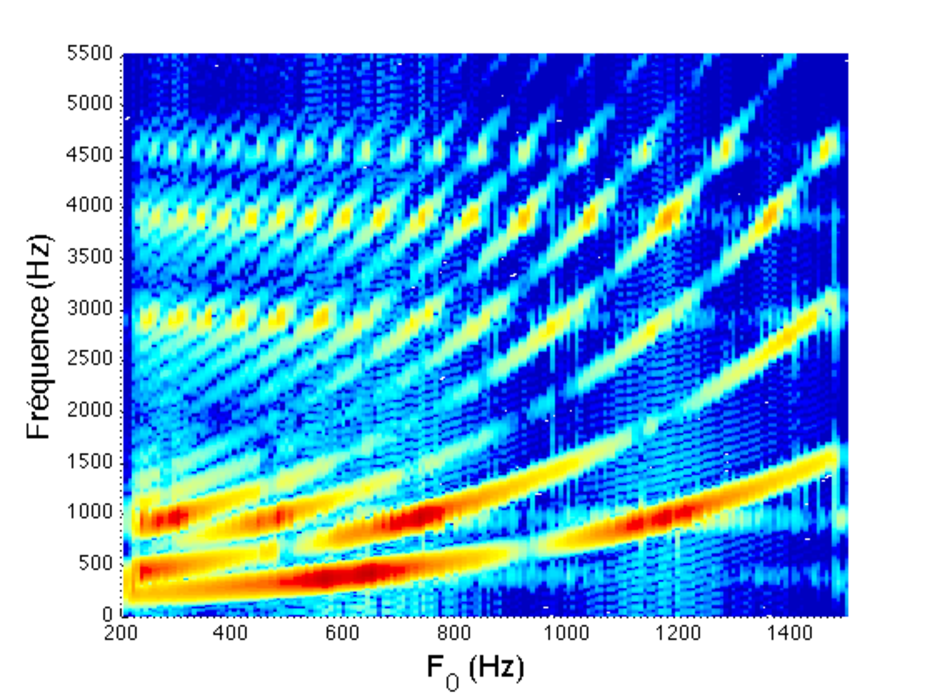
\includegraphics[width=.45\linewidth]{ch2/fig/Fi-F0-dpdce-sans_soprano_u_200-1500Hz_dig13b3.pdf}}
%   \label{Fig:Fi-F0-dpdce_sans}
%   \hspace{0.3cm}
%   \subfloat
% 	[{\it Avec dépendances}]  
%   {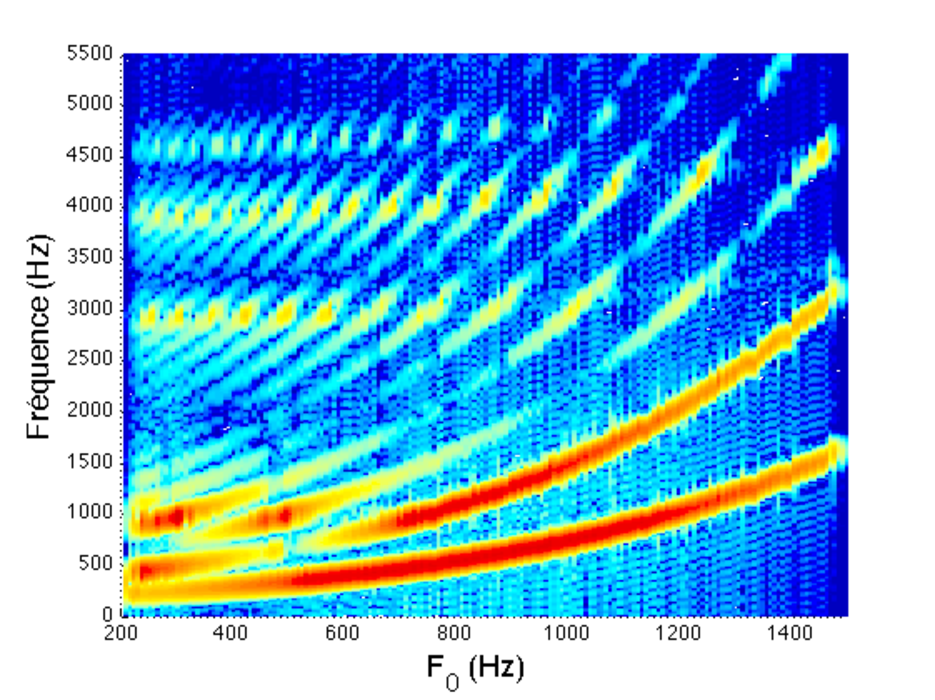
\includegraphics[width=.45\linewidth]{ch2/fig/Fi-F0-dpdce-avec_soprano_u_200-1500Hz_dig13b3.pdf}}
%   \label{Fig:Fi-F0-dpdce_avec}
%     \caption{{\it Spectrogrammes de la voyelle /a/ de synthèse, où $F_0$ augmente avec le temps, (a) sans ou (b) avec les dépendances entre les fréquences centrales des formants et de $F_0$. \textit{Voir fichiers audios~/ vidéos~\ref{fav:fi-f0-dependance}}\\
% }}
%   \label{Fig:Fi-F0-dpdce}
% \end{figure}

% \subsubsection{a) La soufflerie}

% \begin{table}[!h]
% 	\centering
% 	\begin{tabular}{|c|c|c|} 
% 		\hline
% 		& \centering \textbf{Tessiture naturelle moyenne} & \centering \textbf{Tessiture
% dans le synthétiseur} \tabularnewline
% 		\hline
% 		\bf Basse & Mi2-Mi4 & Sol$\sharp$1-Sol4\\
% 		\hline
% 		\bf Ténor & Do3-Si4 & Sol$\sharp$1-Sol4\\
% 		\hline
% 		\bf Alto & Fa3-Mi5 & Sol$\sharp$2-Sol5\\
% 		\hline
% 		\bf Soprano & Si3-Do6 & Sol$\sharp$3-Sol6\\
% 		\hline
% 	\end{tabular}
% 	\caption{\textit{Tessiture des chanteurs naturels et synthétiques (La3=440 Hz). Voir fichiers audios~/ vidéos~\ref{fav:types-voix-1}}}
% 	\label{Tab:tessChant}
% \end{table}

